% !TeX root = RJwrapper.tex
\title{Partitioned Local Depth (PaLD) Clustering Analyses in R}
\author{by Lucy D'Agostino McGowan, Katherine Moore, Kenneth Berenhaut}

\maketitle

\abstract{%
An abstract of less than 150 words.
}

% Any extra LaTeX you need in the preamble

\hypertarget{introduction}{%
\subsection{Introduction}\label{introduction}}

\begin{itemize}
\tightlist
\item
  Describe PaLD (Ken \& Kate?)
\item
  Cite PaLD
\end{itemize}

We present a new package, \CRANpkg{pald}, for calculating partitioned
local depth (PaLD) probabilities, implementing clustering analyses, and
creating data visualizations to represent the clusters. This paper will
describe how to use the package as well as walk through two examples.

\hypertarget{pald}{%
\subsection{pald}\label{pald}}

The main functions in \CRANpkg{pald} package can be split into 3
categories:

\begin{enumerate}
\def\labelenumi{\arabic{enumi}.}
\tightlist
\item
  Helper functions to organize data into the correct format, into
  distance matrices and then contribution matrices
\item
  Functions that convert a contribution matrix into a variety of useful
  formats, including partitioned local depths, clusters, and graphs
\item
  Plotting functions
\end{enumerate}

In addition, the package provides a number of pertinent example data
sets commonly used to demonstrate cluster algorithms, including a
synthetic data set of two-dimensional points created by
\citet{gionis1clustering} to demonstrate clustering aggregation, a
sample of walking distances from a pump in the infamous cholera outbreak
\citep{cholera}, clustering data generated from the scikit-learn Python
package \citep{pedregosa2011scikit}, and data compiled by \cite{tissue}
of tissue gene expressions.

While it is not a necessity, the \CRANpkg{pald} package is designed to
function well with the pipe operator, \texttt{\%\textgreater{}\%}, from
the \citet{magrittr} \CRANpkg{magrittr} package in that the first
argument of each function is the data. This functionality will be
demonstrated below.

\hypertarget{helper-functions-to-create-contribution-matrix}{%
\subsubsection{Helper functions to create contribution
matrix}\label{helper-functions-to-create-contribution-matrix}}

For demonstration purposes, below is a sample data frame with two
variables, \texttt{x1} and \texttt{x2}. The methods put forth here work
on data frames with higher dimensions, as described in the
\textbf{Examples} section, we are simply choosing a small data frame
here for demonstration purposes.

\begin{Schunk}
\begin{Sinput}
library(pald)
d <- data.frame(
  x1 = c(6, 8, 11, 16, 4),
  x2 = c(5, 4, 13, 7, 18)
)
rownames(d) <- c("A", "B", "C", "D", "E")
\end{Sinput}
\end{Schunk}

The first step needed to calculate the partitioned local depths is to
construct a \emph{distance matrix}. If the data are already in this
form, the user can skip to the next step. The
\texttt{get\_distance\_matrix()} function converts an input data frame
into a distance matrix, as demonstrated below.

\begin{Schunk}
\begin{Sinput}
get_distance_matrix(d)
\end{Sinput}
\begin{Soutput}
#>           A         B        C        D        E
#> A 0.0000000 0.4584177 1.717380 2.158418 2.229205
#> B 0.4584177 0.0000000 1.644296 1.778777 2.505929
#> C 1.7173802 1.6442957 0.000000 1.468398 1.713327
#> D 2.1584182 1.7787772 1.468398 0.000000 3.158040
#> E 2.2292047 2.5059291 1.713327 3.158040 0.000000
\end{Soutput}
\end{Schunk}

This will create an \(n\times n\) distance matrix, where \(n\)
corresponds to the number of observations in the original data frame, in
this example \(n = 5\). By default, the distance matrix is
\emph{scaled}, is possible to create a distance matrix that is not
scaled by changing the \texttt{scale} argument to \texttt{FALSE}.

\begin{Schunk}
\begin{Sinput}
get_distance_matrix(d, scale = FALSE)
\end{Sinput}
\begin{Soutput}
#>           A         B        C         D         E
#> A  0.000000  2.236068 9.433981 10.198039 13.152946
#> B  2.236068  0.000000 9.486833  8.544004 14.560220
#> C  9.433981  9.486833 0.000000  7.810250  8.602325
#> D 10.198039  8.544004 7.810250  0.000000 16.278821
#> E 13.152946 14.560220 8.602325 16.278821  0.000000
\end{Soutput}
\end{Schunk}

As mentioned previously, the functions in this package are designed to
work with the \CRANpkg{magrittr} pipe operator,
\texttt{\%\textgreater{}\%}, so the same code as above could be written
utilizing this format.

\begin{Schunk}
\begin{Sinput}
d %>%
  get_distance_matrix()
\end{Sinput}
\begin{Soutput}
#>           A         B        C        D        E
#> A 0.0000000 0.4584177 1.717380 2.158418 2.229205
#> B 0.4584177 0.0000000 1.644296 1.778777 2.505929
#> C 1.7173802 1.6442957 0.000000 1.468398 1.713327
#> D 2.1584182 1.7787772 1.468398 0.000000 3.158040
#> E 2.2292047 2.5059291 1.713327 3.158040 0.000000
\end{Soutput}
\end{Schunk}

This distance matrix can then be passed to the
\texttt{get\_contribution\_matrix()} function in order to calculate a
matrix of contributions. Again, if the user begins with a distance
matrix, they can skip the first step and simple input the contribution
matrix into this function.

\begin{Schunk}
\begin{Sinput}
distance_matrix <- get_distance_matrix(d)
get_contribution_matrix(distance_matrix)
\end{Sinput}
\begin{Soutput}
#>        1      2     3     4      5
#> A 0.2875 0.1625 0.000 0.050 0.0000
#> B 0.1750 0.3000 0.050 0.050 0.0000
#> C 0.0000 0.0625 0.300 0.175 0.0500
#> D 0.0500 0.0500 0.175 0.300 0.0000
#> E 0.0000 0.0000 0.050 0.000 0.2125
\end{Soutput}
\end{Schunk}

Again, the \CRANpkg{magrittr} pipe can be used as follows.

\begin{Schunk}
\begin{Sinput}
d %>%
  get_distance_matrix() %>%
  get_contribution_matrix()
\end{Sinput}
\begin{Soutput}
#>        1      2     3     4      5
#> A 0.2875 0.1625 0.000 0.050 0.0000
#> B 0.1750 0.3000 0.050 0.050 0.0000
#> C 0.0000 0.0625 0.300 0.175 0.0500
#> D 0.0500 0.0500 0.175 0.300 0.0000
#> E 0.0000 0.0000 0.050 0.000 0.2125
\end{Soutput}
\end{Schunk}

The \emph{contribution matrix} output by the
\texttt{get\_contribution\_matrix()} is the main input for the majority
of the remaining functions.

\hypertarget{functions-that-convert-a-contribution-matrix-into-useful-formats}{%
\subsubsection{Functions that convert a contribution matrix into useful
formats}\label{functions-that-convert-a-contribution-matrix-into-useful-formats}}

From the \emph{contribution matrix}, a variety of useful quantities can
be calculated. Below, we create a contribution matrix using the
functions described in the previous section.

\begin{Schunk}
\begin{Sinput}
d %>%
  get_distance_matrix() %>%
  get_contribution_matrix() -> contribution_matrix
\end{Sinput}
\end{Schunk}

To calculate the \emph{clusters} that each point will fall into, we can
use the \texttt{get\_clusters()} function. This will output a data frame
with two columns, the first will correspond to the \texttt{point}, as
identified by the row name of the original input data frame, \texttt{d},
the second will identify the \texttt{cluster} that each point belongs
to.

\begin{Schunk}
\begin{Sinput}
get_clusters(contribution_matrix)
\end{Sinput}
\begin{Soutput}
#> # A tibble: 5 x 2
#>   point cluster
#>   <chr>   <dbl>
#> 1 A           1
#> 2 B           1
#> 3 C           2
#> 4 D           2
#> 5 E           3
\end{Soutput}
\end{Schunk}

In this example, three clusters are identified with these five points.
Points \texttt{A} and \texttt{B} fall into cluster 1. Points \texttt{C}
and \texttt{D} into cluster 2, and point \texttt{E} in cluster 3.

The \texttt{get\_depths()} function calculates the \emph{depths} of each
point, outputting a data frame with two columns, \texttt{point}
indicating the point, as identified by the row name of the original data
frame, \texttt{d}, and \texttt{depth} indicating the depth of the point.
The data frame is arranged by depth, with the deepest point listed
first.

\begin{Schunk}
\begin{Sinput}
get_depths(contribution_matrix)
\end{Sinput}
\begin{Soutput}
#> # A tibble: 5 x 2
#>   point depth
#>   <chr> <dbl>
#> 1 C     0.588
#> 2 B     0.575
#> 3 D     0.575
#> 4 A     0.5  
#> 5 E     0.262
\end{Soutput}
\end{Schunk}

In this case, the deepest point is \texttt{C}.

The \texttt{get\_bound()} function will calculate the \emph{bound} of
the contribution matrix.

\begin{Schunk}
\begin{Sinput}
get_bound(contribution_matrix)
\end{Sinput}
\begin{Soutput}
#> [1] 0.14
\end{Soutput}
\end{Schunk}

In this case, the bound is 0.14.

The \texttt{any\_isolated()} function will check whether there are any
isolated points that will inadvertently be dropped by a graph.

\begin{Schunk}
\begin{Sinput}
any_isolated(contribution_matrix)
\end{Sinput}
\begin{Soutput}
#> [1] FALSE
\end{Soutput}
\end{Schunk}

In this case, there are no isolated points.

The \texttt{get\_pald\_cluster\_matrix()} will calculate a matrix of
partitioned local depth clusters. This function contains an argument
\texttt{keep\_all\_edges} that indicates whether all edges should be
kept. The default value is \texttt{FALSE}, indicating that edges that
are less than the expectation will be dropped, allowing a clear
clustering of points. Changing this argument to \texttt{TRUE} results in
the pairwise minimum of the contribution matrix and the transpose of the
contribution matrix.

\begin{Schunk}
\begin{Sinput}
get_pald_cluster_matrix(contribution_matrix, keep_all_edges = TRUE)
\end{Sinput}
\begin{Soutput}
#>        1      2     3     4      5
#> A 0.2875 0.1625 0.000 0.050 0.0000
#> B 0.1625 0.3000 0.050 0.050 0.0000
#> C 0.0000 0.0500 0.300 0.175 0.0500
#> D 0.0500 0.0500 0.175 0.300 0.0000
#> E 0.0000 0.0000 0.050 0.000 0.2125
\end{Soutput}
\end{Schunk}

Leaving the \texttt{keep\_all\_edges} as the default, \texttt{FALSE}
will take this pairwise minimum seen above and drop the edges that are
less than the expectation.

\begin{Schunk}
\begin{Sinput}
get_pald_cluster_matrix(contribution_matrix)
\end{Sinput}
\begin{Soutput}
#>        1      2     3     4 5
#> A 0.0000 0.1625 0.000 0.000 0
#> B 0.1625 0.0000 0.000 0.000 0
#> C 0.0000 0.0000 0.000 0.175 0
#> D 0.0000 0.0000 0.175 0.000 0
#> E 0.0000 0.0000 0.000 0.000 0
\end{Soutput}
\end{Schunk}

Finally, the \texttt{get\_pald\_graph()} function takes the contribution
matrix and creates an \CRANpkg{igraph} object, a graph that describes
the relationship between the points.

\begin{Schunk}
\begin{Sinput}
get_pald_graph(contribution_matrix)
\end{Sinput}
\begin{Soutput}
#> IGRAPH 2c0b54a UNW- 5 2 -- 
#> + attr: name (v/c), weight (e/n)
#> + edges from 2c0b54a (vertex names):
#> [1] A--B D--C
\end{Soutput}
\end{Schunk}

Here we see that there are two connected components, points \texttt{A}
and \texttt{B}, which form the first cluster, and points \texttt{D} and
\texttt{C} which form the second.

\hypertarget{plotting-functions}{%
\subsection{Plotting functions}\label{plotting-functions}}

The final category of function is functions for data visualization. We
can begin by visualizing the points in data frame \texttt{d} (Figure
\ref{fig:fig1}).

\begin{Schunk}
\begin{Sinput}
library(ggplot2)
ggplot(d, aes(x1, x2)) +
  geom_text(label = rownames(d))
\end{Sinput}
\begin{figure}
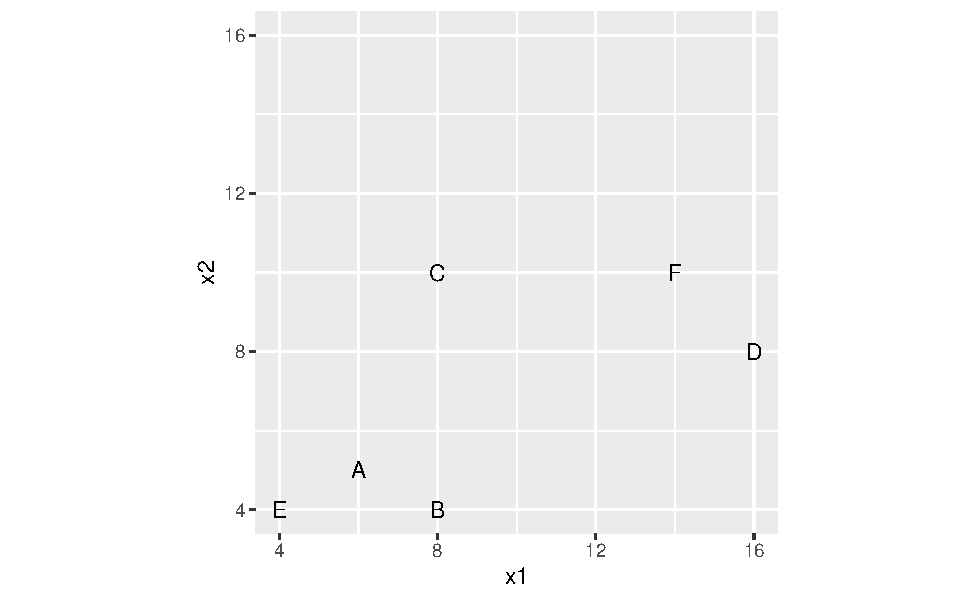
\includegraphics{manuscript_files/figure-latex/fig1-1} \caption[Visualize the points from data frame `d`]{Visualize the points from data frame `d`}\label{fig:fig1}
\end{figure}
\end{Schunk}

We can then pass the contribution matrix to the
\texttt{plot\_pald\_graph()} function to view the relationship between
points (Figure \ref{fig:fig2}). By default, this will invoke the
\texttt{layout\_nicely()} function from \CRANpkg{igraph} to determine
the layout of the graph.

\begin{Schunk}
\begin{Sinput}
d %>%
  get_distance_matrix() %>%
  get_contribution_matrix() %>%
  plot_pald_graph()
\end{Sinput}
\begin{figure}
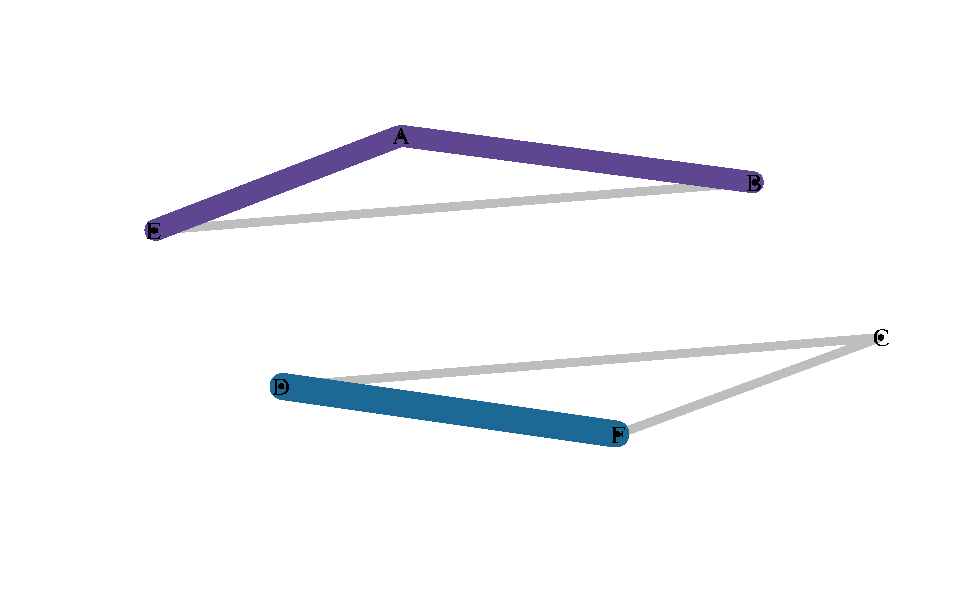
\includegraphics{manuscript_files/figure-latex/fig2-1} \caption[PaLD graph displaying the relationship between the points in data frame `d`]{PaLD graph displaying the relationship between the points in data frame `d`}\label{fig:fig2}
\end{figure}
\end{Schunk}

The \texttt{layout} argument allows the user to pass a matrix to dictate
the layout of the graph. For example, if we wanted the graph to match
the visualization displayed in Figure \ref{fig:fig1}, we can pass
\texttt{as.matrix(d)}, or a matrix of the data frame \texttt{d} to the
\texttt{layout} argument (Figure \ref{fig:fig3}.

\begin{Schunk}
\begin{Sinput}
d %>%
  get_distance_matrix() %>%
  get_contribution_matrix() %>%
  plot_pald_graph(layout = as.matrix(d))
\end{Sinput}
\begin{figure}
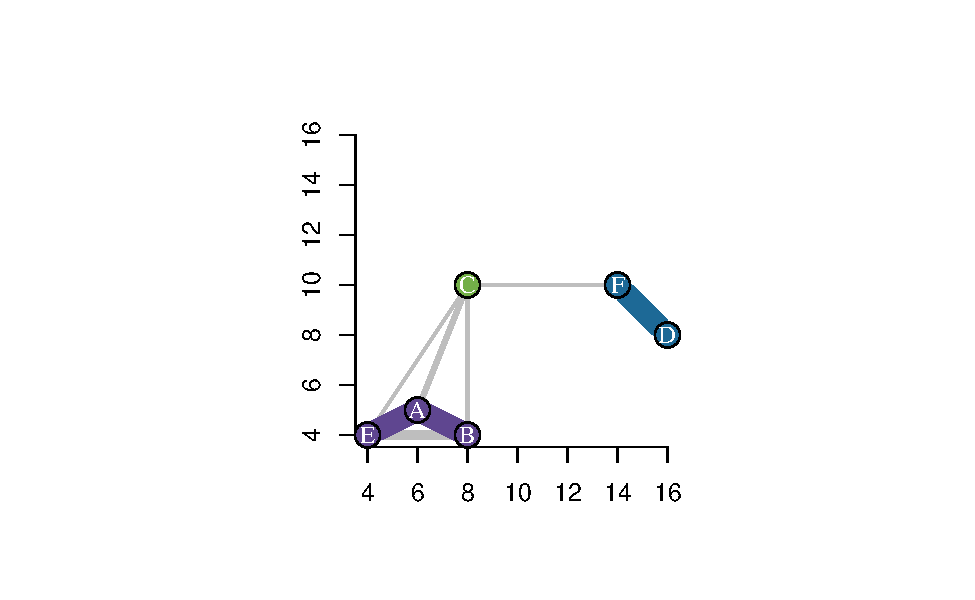
\includegraphics{manuscript_files/figure-latex/fig3-1} \caption[PaLD graph displaying the relationship between the points in data frame `d`, matching the original layout in Figure 1]{PaLD graph displaying the relationship between the points in data frame `d`, matching the original layout in Figure 1}\label{fig:fig3}
\end{figure}
\end{Schunk}

This \texttt{plot\_pald\_graph()} function will also permit parameters
that can be passed to the \texttt{plot.igraph()} function. For example,
to add axes to the graph, the user can pass the \texttt{axes\ =\ TRUE}
argument to the \texttt{...} in the \texttt{plot\_pald\_graph()}
function (Figure \ref{fig:fig4}).

\begin{Schunk}
\begin{Sinput}
d %>%
  get_distance_matrix() %>%
  get_contribution_matrix() %>%
  plot_pald_graph(layout = as.matrix(d),
                  axes = TRUE)
\end{Sinput}
\begin{figure}
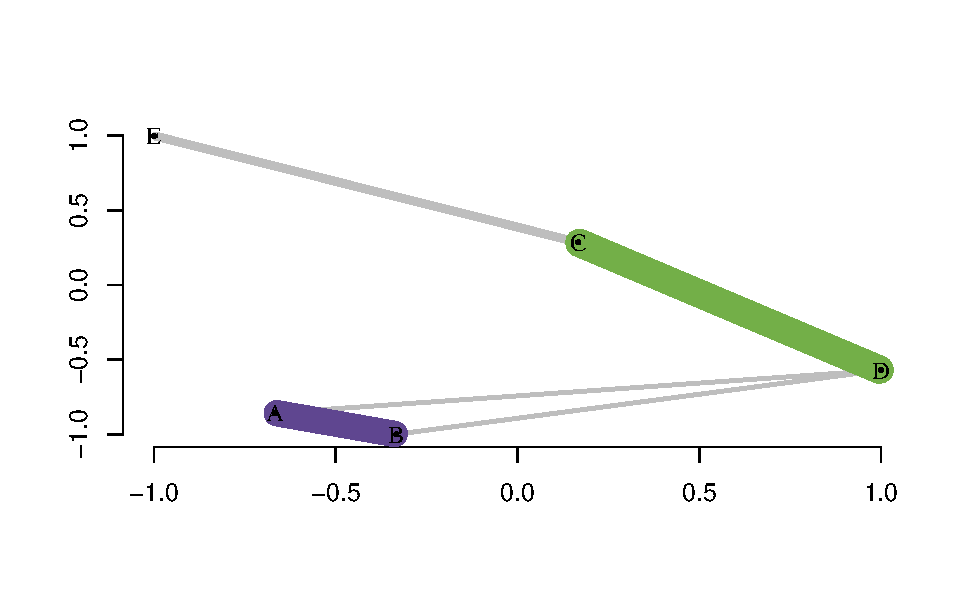
\includegraphics{manuscript_files/figure-latex/fig4-1} \caption[PaLD graph displaying the relationship between the points in data frame `d`, matching the original layout in Figure 1, adding axes]{PaLD graph displaying the relationship between the points in data frame `d`, matching the original layout in Figure 1, adding axes}\label{fig:fig4}
\end{figure}
\end{Schunk}

\hypertarget{examples}{%
\subsection{Examples}\label{examples}}

We will demonstrate the utility of the \CRANpkg{pald} package in two
clustering examples.

\hypertarget{clustering-tissue-gene-expression-data}{%
\subsubsection{Clustering tissue gene expression
data}\label{clustering-tissue-gene-expression-data}}

The first example data frame is a subset of tissue gene expression data
from \citet{zilliox2007gene}, \citet{mccall2011gene}, and
\citet{mccall2014gene}, obtained from the \textbf{tissuesGeneExpression}
bioconductor package \citep{tissue}. This data set is included in the
\CRANpkg{pald} package in an object called \texttt{tissue}.

The \texttt{tissue} object is a matrix with 189 rows, each with a
corresponding tissue, such as \texttt{colon}, \texttt{kidney} or
\texttt{cerebellum}. There are 22,215 columns corresponding to gene
expression data from each of these rows.

We will first calculate the contribution matrix for this data frame.

\begin{Schunk}
\begin{Sinput}
tissue_contribution_matrix <- tissue %>%
  get_distance_matrix(scale = FALSE) %>%
  get_contribution_matrix()
\end{Sinput}
\end{Schunk}

We can then use this contribution matrix to display the relationship
between tissue samples using the \texttt{plot\_pald\_graph()} function
(Figure \ref{fig:fig5}).

\begin{Schunk}
\begin{Sinput}
plot_pald_graph(tissue_contribution_matrix)
\end{Sinput}
\begin{figure}
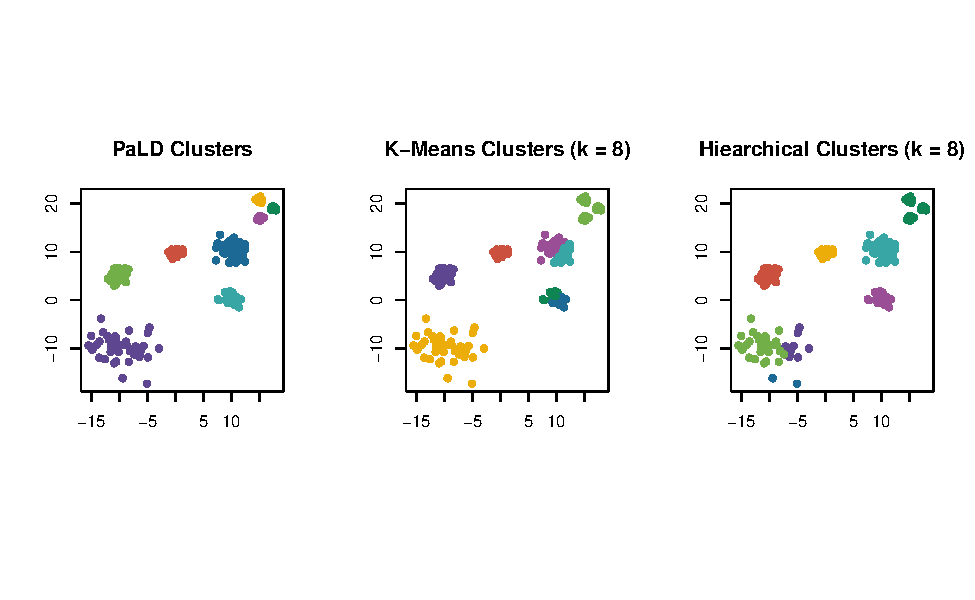
\includegraphics{manuscript_files/figure-latex/fig5-1} \caption[PaLD clustering of tissue data]{PaLD clustering of tissue data}\label{fig:fig5}
\end{figure}
\end{Schunk}

The \texttt{get\_clusters()} function can be used to identify the
clusters of each tissue sample. Since the output is a data frame, we can
summarize the clusters using commonly used data analysis techniques. For
demonstration purposes, we will use the \CRANpkg{dplyr} package to
summarize the contribution of clusters.

\begin{Schunk}
\begin{Sinput}
library(dplyr)
get_clusters(tissue_contribution_matrix) %>%
  group_by(cluster, point) %>%
  count()
\end{Sinput}
\begin{Soutput}
#> # A tibble: 19 x 3
#> # Groups:   cluster, point [19]
#>    cluster point           n
#>      <dbl> <chr>       <int>
#>  1       1 endometrium    15
#>  2       1 kidney         39
#>  3       2 hippocampus    31
#>  4       3 cerebellum     26
#>  5       4 cerebellum      1
#>  6       5 colon          33
#>  7       6 colon           1
#>  8       7 liver           7
#>  9       8 cerebellum      1
#> 10       9 liver          17
#> 11      10 cerebellum      2
#> 12      11 liver           2
#> 13      12 cerebellum      1
#> 14      13 cerebellum      4
#> 15      14 cerebellum      2
#> 16      15 cerebellum      1
#> 17      16 placenta        2
#> 18      17 placenta        1
#> 19      18 placenta        3
\end{Soutput}
\end{Schunk}

From this, we can glean that cluster one consists of two types of
tissue, the kidney and endometrium. Cluster two is comprised of only the
hippocampus.

\hypertarget{clustering-generated-data}{%
\subsubsection{Clustering generated
data}\label{clustering-generated-data}}

The \CRANpkg{pald} includes two data frames generated from the
scikit-learn Python package \citep{pedregosa2011scikit},
\texttt{noisy\_moons} and \texttt{noisy\_circles}.

The \texttt{noisy\_moons} data frame consists of 500 rows and two
columns.

\begin{Schunk}
\begin{Sinput}
moons_contribution_matrix <- noisy_moons %>%
  get_distance_matrix() %>%
  get_contribution_matrix()
\end{Sinput}
\end{Schunk}

When plotting the \texttt{noisy\_moons} PaLD graph, we want the layout
to match the layout of the original data, so we will pass
\texttt{as.matrix(noisy\_moons)} to the \texttt{layout} parameter in the
\texttt{plot\_pald\_graph()} function. Additionally, here the row names
are meaningless, they just correspond to the location of the generated
data, so we can remove the labels on the plot by passing
\texttt{vertex.label\ =\ NA} to the \texttt{...} of the
\texttt{plot\_pald\_graph()} function.

\begin{Schunk}
\begin{Sinput}
plot_pald_graph(moons_contribution_matrix,
                layout = as.matrix(noisy_moons),
                vertex.label = NA)
\end{Sinput}
\end{Schunk}

The \texttt{noisy\_circles} data frame consists of 500 rows and two
columns. We can create the contribution matrix for this data frame using
the same methods as used for the \texttt{noisy\_moons} data.

\begin{Schunk}
\begin{Sinput}
circles_contribution_matrix <- noisy_circles %>%
  get_distance_matrix() %>%
  get_contribution_matrix()
\end{Sinput}
\end{Schunk}

Similarly, we will pass the layout and remove vertex labels for the
noisy circles PaLD plot.

\begin{Schunk}
\begin{Sinput}
plot_pald_graph(circles_contribution_matrix,
                layout = as.matrix(noisy_circles),
                vertex.label = NA)
\end{Sinput}
\end{Schunk}

Because these are \CRANpkg{igraph} objects, they can be combined as you
would normally combine a plot. For example, we could add the line
\texttt{par(mfrow\ =\ c(1,\ 2))} above the plot calls to create an
output where both plots are displayed side by side (Figure
\ref{fig:fig6}).

\begin{Schunk}
\begin{Sinput}
par(mfrow = c(1, 2))
plot_pald_graph(moons_contribution_matrix,
                layout = as.matrix(noisy_moons),
                vertex.label = NA)
plot_pald_graph(circles_contribution_matrix,
                layout = as.matrix(noisy_circles),
                vertex.label = NA)
\end{Sinput}
\begin{figure}
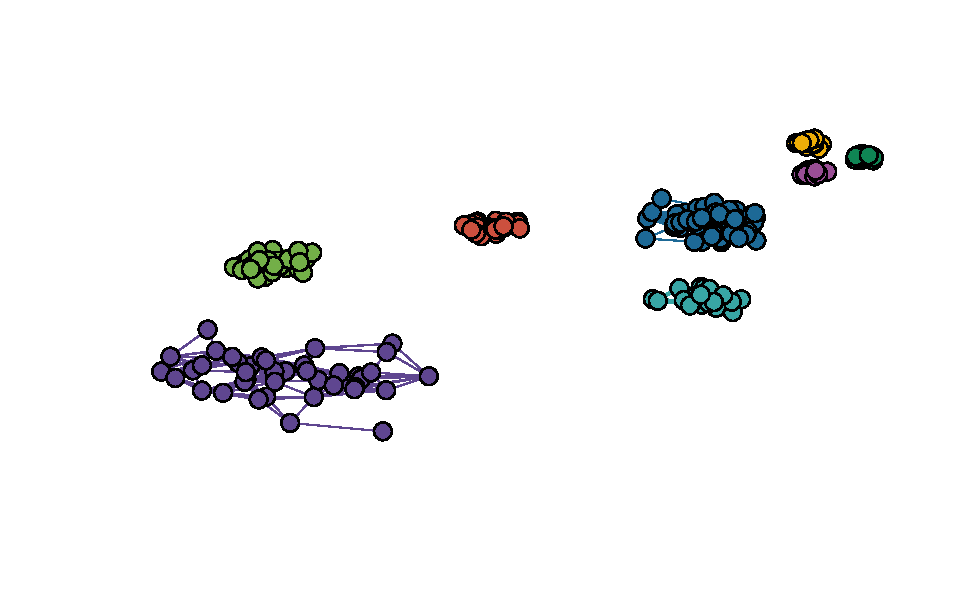
\includegraphics{manuscript_files/figure-latex/fig6-1} \caption[PaLD clustering of noisy moons (left) and noisy circles (right) data]{PaLD clustering of noisy moons (left) and noisy circles (right) data}\label{fig:fig6}
\end{figure}
\end{Schunk}

The ability of the PaLD algorithm to discern clusters is demonstrated
here.

\hypertarget{summary}{%
\subsection{Summary}\label{summary}}

This paper introduces the \CRANpkg{pald} package, demonstrating it's
utility for providing a parameter-free clustering algorithm that can
easily be applied to any data set.

\bibliography{RJreferences}


\address{%
Lucy D'Agostino McGowan\\
Wake Forest University\\
Winston-Salem, NC\\ 27106\\
}
\href{mailto:mcgowald@wfu.edu}{\nolinkurl{mcgowald@wfu.edu}}

\address{%
Katherine Moore\\
Wake Forest Unversity\\
Winston-Salem, NC\\ 27106\\
}
\href{mailto:mooreke@wfu.edu}{\nolinkurl{mooreke@wfu.edu}}

\address{%
Kenneth Berenhaut\\
Wake Forest University\\
Winston-Salem, NC\\ 27106\\
}
\href{mailto:berenhks@wfu.edu}{\nolinkurl{berenhks@wfu.edu}}

